%%
%%
\documentclass[12pt]{book}
\usepackage{amsfonts,amssymb,amsmath,amsthm}
\usepackage{graphicx}
\usepackage{hyperref}
\usepackage{boxedminipage}
\usepackage{geometry}
\usepackage{array}
\usepackage{enumitem}

\newcolumntype{C}[1]{>{\centering\let\newline\\\arraybackslash\hspace{0pt}}m{#1}}

\setlength{\textheight}{10in}
\setlength{\textwidth}{7.4in}
\setlength{\topmargin}{-0.75in}
\setlength{\oddsidemargin}{-0.7in}
\setlength{\evensidemargin}{-0.7in}
\setlength{\parskip}{0.15in}
\setlength{\parindent}{0in}


\begin{document}


\vspace{-1.0in}\begin{center}
\Large{MCV4U : Calculus and Vectors}\\
\Large{MCV4UR : Advanced Placement Calculus and Vectors }

\Large{Assignment \#2}


\end{center}

%\medskip

\vspace{0.015in}\hrulefill\ 

\textbf{Reference Declaration} %  Fill in your Reference Declarations in this section before your submit your assignment.

Complete the Reference Declaration section below in order for your assigment to be graded.

If you used any references beyond the course text and lectures (such as other texts, discussions with colleagues or online resources), indicate this information in the space below.  If you did not use any aids, state this in the space provided. 

Be sure to cite appropriate theorems throughout your work. You may use shorthand for well-known theorems like the FT, RRT, MVT, IVT, etc. 

Note: Your submitted work must be \textbf{your original work}. 

Family Name: Wong\\%Family Name Here
First Name: Max%First Name Here

Declared References: 

Used WolframAlpha to confirm some calculations \textbf{ as a check }.

% Type your references here.
% You can use as many lines as required.

\vspace{0.015in}\hrulefill\ 

\newpage

% INSTRUCTIONS SECTION
\section*{Instructions}

\begin{center}
\setlength{\fboxrule}{2pt}
\begin{boxedminipage}{6.5in}
1.	Organize and express complete, effective and concise responses to each problem.\\
2.	Use appropriate mathematical conventions and notation wherever possible.\\
3.	Provide logical reasoning for your arguments and cite any relevant theorems. \\
4.  The quality of your communication will be heavily weighted.
\end{boxedminipage}
\end{center} 

% EVALUATION SECTION
\section*{Evaluation}

% LEARNING EXPECTATION(S)
\begin{itemize}
\item Students will demonstrate an understanding of derivative rules and use them to solve problems.
\end{itemize}

% RUBRIC
\begin{tabular}{| C{2in} | C{1in} | C{1in} | C{1in} | C{1in} |}
\hline
\textbf{Criteria} & \textbf{Level 1} & \textbf{Level 2} & \textbf{Level 3} & \textbf{Level 4} \\
\hline
\emph{Understanding of Mathematical Concepts} & Demonstrates limited understanding & Demonstrates some understanding & Demonstrates considerable understanding & Demonstrates thorough understanding of concepts \\
\hline
\emph{Selecting Tools and Strategies} & Selects and applies appropriate tools and strategies, with major errors, omissions, or mis-sequencing & Selects and applies appropriate tools and strategies, with minor errors, omissions, or mis-sequencing & Selects and applies appropriate tools and strategies accurately, and in a logical sequence & Selects and applies appropriate and efficient tools and strategies accurately to create mathematically elegant solutions \\
\hline
\emph{Reasoning and Proving} & Inconsistently or erroneously employs logic to develop and defend statements & Statements are developed and defended with some omissions or leaps in logic & Frequently develops and defends statements with reasonable logical justification & Consistently develops and defends statements with sophisticated and/or complete logical justification \\
\hline
\emph{Communicating} & Expresses and organizes mathematical thinking with limited effectiveness & Expresses and organizes mathematical thinking with some effectiveness & Expresses and organizes mathematical thinking with considerable effectiveness & Expresses and organizes mathematical thinking with a high degree of effectiveness \\
\hline
\end{tabular}

\pagebreak



%%%%%%%%%%%% PROBLEMS START HERE

\textbf{Instructions:} Answer True or False to the following statements.

\begin{enumerate}
\item  If $f$ and $g$ are differentiable then $\frac{d}{dx} (f+g) = f' + g'$.
\item If $f$ and $g$ are differentiable then $\frac{d}{dx} (fg) = f'g+2f'g'+fg'$.
\item If $f$ and $g$ are differentiable then $\frac{d}{dx} (f(g(x)) = f'(g(x)) \cdot g'(x)$.
\item If $f$ is differentiable then $\frac{d}{dx} (\sqrt{f(x)}) = \frac{f'(x)}{2\sqrt{x}}$.
\item The derivative of a polynomial function is a polynomial function.
\item The derivative of a rational function is a rational function.
\item The derivative of an exponential function is an exponential function.
\item The derivative of a sinusoidal function is a sinusoidal function.
\item The derivative of a logarithmic function is a logarithmic function.
\item If $f(x) = (x^p - 1)^q$ where $p,q \in \mathbb{Z^+}$ then $-1 \le f^{(pq+1)}(x) \le +1$.
\item If $f'(c)=0$, then $f$ has a local maximum or minimum at $x=c$.
\item If $f$ has an absolute minimum at $x=c$ then $f'(c) = 0$. 
\item If $f$ and $g$ are increasing on an interval $I$ then $f+g$ is also increasing on $I$.
\item If $f$ and $g$ are increasing on an interval $I$ then $fg$ is also increasing on $I$.
\item If $f$ is periodic then $f'$ is periodic.
\item If $f$ is even then $f'$ is odd.
\item There exists a function $g$ such that $g(x)>0$, $g'(x)<0$, and $g''(x)>0$ for all $x \in \mathbb{R}$.
\item There exists a function $h$ such that $h(x)<0$, $h'(x)<0$, and $h''(x)>0$ for all $x \in \mathbb{R}$.
\item If $f(x)=\sin(x)$ then the least value of $n \in \mathbb{Z^+}$ such that $f^{(n)}(x) = f(x)$ is $n=4$.
\item If $f'(x) = g'(x) $ for $0 < x < 1$ then $f(x) = g(x)$ for $0 < x < 1$.
\newpage

\section*{True-False Answers}

\begin{enumerate}[label={\arabic*.}]
\item true
\item false
\item true
\item false
\item true %Is linear or constant a polynomial?
\item true
\item true
\item true %sinosoidal are periodic, no disconc.
\item false
\item true
\item false
\item false %
\item true
\item true
\item true
\item true
\item true
\item false %
\item true
\item false
\end{enumerate}

Fill in your responses to the True-False questions above. Be sure to use only capital T or F.

\newpage

%% PROBLEM 21
\item \textbf{Prove} that the tangent lines to the graph of the function $y=ax^2+bx+c$, where $a,b,c \in \mathbb{R}, a\neq 0$, at any two points with x-coordinates $p$ and $q$, where $p,q \in \mathbb{R}$, must intersect at a point whose x-coordinate is $\dfrac{p+q}{2}$.

\vspace{0.3cm} 
\textbf{Solution to Question 21:}\\
 What we need to do is solve for the equations of the 2 tangent lines 
 (linear equations), then solve their intercept. Consider the constant 
 k. This is a stand-in for p or q. Pretty much $k \in \mathbb{R}$. Let's 
 try and solve for the slope first. We know that the slope comes from the 
 derivative evaluated at a certain point, like k.

 \addtolength{\jot}{1em}
\begin{align*}
    y &= ax^2+bx+c && \text{base quadratic function} \\
    y' &= 2ax+b && \text{Get derivative} \\
    y' &= 2ak+b && \text{Evaluate at x=k} \\
\end{align*}

\vspace{-1cm}
Now that we have our slope, we can substitute the slope into the standard 
linear equation $y=mx+i$. where m represents the slope and i (because b is 
already used) represents the y-intercept. Next, we need to determine the 
y-intercept. We can find i by evaluating the linear equation at a point (x,y) 
and isolate for i. First, we need to find a point. Given the $x=k$, we can say the following:

\vspace{-0.3cm}
\addtolength{\jot}{0.4em}
\begin{align*}
    y &= ax^2+bx+c && \text{base quadratic function} \\
    y &= ak^2+bk+c && \text{Evaluate at x=k} \\
\end{align*}

\vspace{-1cm}
With the coordinate $(k,ak^2+bk+c)$, which is where the tangent line 
meets the quadratic equation, we can now solve for i:

\vspace{-0.3cm}
\addtolength{\jot}{0.3em}
\begin{align*}
    y &= mx + i && \text{standard linear equation formula} \\
    y &= (2ak+b)x + i && \text{Substitute slope in } m = 2ak+b \\
    ak^2+bk+c &= (2ak+b)k + i && \text{Substitute coordinate in } (x,y) = (k,ak^2+bk+c) \\
    ak^2+bk+c &= 2ak^2+bk + i && \text{Expand} \\
    ak^2+bk+c - 2ak^2 - bk &= i && \text{Simplify} \\
    -ak^2+c &= i && \text{Simplify} \\
\end{align*}

\newpage

Therefore, now that we have the y-intercept, we can substitute 
this back into the linear equation. We now have $y = (2ak+b)x - ak^2+c$. 
Since k was a fill in for p and q, why dont we re-evaluate the linear equation 
found using p and q. 

\[ \begin{cases} 
    y = (2aq+b)x - aq^2+c & \textbf{(1)} \text{\space \space \space} k=p \\
    y = (2aq+b)x - aq^2+c & \textbf{(2)} \text{\space \space \space} k=q
 \end{cases}
\]

Now solve by substituting one into the other using y. Isolating 
for x will result in the x-coordinate of the intercept.

\vspace{-0.3cm}
\addtolength{\jot}{0.3em}
\begin{align*}
    (2ap+b)x - ap^2+c &= (2aq+b)x - aq^2+c && \text{Sub (1) into (2) as y} \\
    2apx+bx - ap^2+c &= 2aqx+bx - aq^2+c && \text{Expand} \\
    2apx - ap^2 &= 2aqx - aq^2 && \text{Simplify} \\
    2px - p^2 &= 2qx - q^2 && \text{Divide all by a} \\
    2px - 2qx &=  - q^2 + p^2 && \text{Subtract } 2qx \text{ and } p^2 \text{ from both sides} \\
    2x(p-q) &=  - q^2 + p^2 && \text{factor 2x} \\
    x &=  \dfrac{- q^2 + p^2}{2(p-q)} && \text{Divide all by 2(p-q)} \\
    x &=  \dfrac{p^2 - q^2}{2(p-q)} && \text{Rearrange numerator} \\
    x &=  \dfrac{(p+q)(p-q)}{2(p-q)} &&  \text{Quadtratic identity} p^2 - q^2 = (p+q)(p-q)\\
    x &=  \dfrac{p+q}{2} &&  \text{Simplify} \qed\\
\end{align*}

\vspace{-1cm}

$\boxed{\text{Therefore the original statement from the question is correct.}}$
If 2 tangent lines are taken from $y=ax^2+bx+c$ at x = q and p, 
the tangents will intersect at x =  p+q/2.
 
\vspace{0.3cm}


\newpage


%% PROBLEM 22
\item \textbf{Determine} the derivative of the function $f(x) = \ln\left( \dfrac{xe^{-x} + \sin(4x)}{1 + 6\sqrt{2x}} \right)$. Go one step at a time and justify each step. Do \emph{not} simplify your answer.

\textbf{Solution to Question 22:}\\
\vspace{-0.5cm} 

\begin{scriptsize}

%\addtolength{\jot}{1em}
\begin{align*}
    f(x) &= \ln\left( \dfrac{xe^{-x} + \sin(4x)}{1 + 6\sqrt{2x}} \right) \\
    f'(x) &= \dfrac{1}{\dfrac{xe^{-x} + \sin(4x)}{1 + 6\sqrt{2x}}} \times \dfrac{d}{dx}\left( \dfrac{xe^{-x} + \sin(4x)}{1 + 6\sqrt{2x}} \right) && \text{Chain Rule}\\
     &= \dfrac{1 + 6\sqrt{2x}}{xe^{-x} + \sin(4x)} \times \dfrac{d}{dx}\left( \dfrac{xe^{-x} + \sin(4x)}{1 + 6\sqrt{2x}} \right) && \text{Simplify}\\
     &= \dfrac{1 + 6\sqrt{2x}}{xe^{-x} + \sin(4x)} \times \dfrac{\dfrac{d}{dx}(xe^{-x} + \sin(4x))(1 + 6\sqrt{2x}) - (xe^{-x} + \sin(4x))\dfrac{d}{dx}(1 + 6\sqrt{2x})}{(1 + 6\sqrt{2x})^2} && \text{Quotient Rule}\\
     &= \dfrac{1 + 6\sqrt{2x}}{xe^{-x} + \sin(4x)} \times \dfrac{\left( \dfrac{d}{dx}xe^{-x} + \dfrac{d}{dx}\sin(4x) \right)(1 + 6\sqrt{2x}) - (xe^{-x} + \sin(4x))(\dfrac{d}{dx}1 + \dfrac{d}{dx}6\sqrt{2x})}{(1 + 6\sqrt{2x})^2} && \text{Distrubute derivative}\\
     &= \dfrac{1 + 6\sqrt{2x}}{xe^{-x} + \sin(4x)} \times \dfrac{\left( \dfrac{d}{dx}xe^{-x} + \dfrac{d}{dx}\sin(4x) \right)(1 + 6\sqrt{2x}) - (xe^{-x} + \sin(4x))(\dfrac{d}{dx}6\sqrt{2x})}{(1 + 6\sqrt{2x})^2} && \text{Apply derivative to 1}\\
     &= \dfrac{1 + 6\sqrt{2x}}{xe^{-x} + \sin(4x)} \times \dfrac{\left( \dfrac{d}{dx}xe^{-x} + \dfrac{d}{dx}4x \times \cos(4x) \right)(1 + 6\sqrt{2x}) - (xe^{-x} + \sin(4x))(\dfrac{d}{dx}6\sqrt{2x})}{(1 + 6\sqrt{2x})^2} && \text{Chain Rule to sin(4x)}\\
     &= \dfrac{1 + 6\sqrt{2x}}{xe^{-x} + \sin(4x)} \times \dfrac{\left( \dfrac{d}{dx}xe^{-x} + 4\cos(4x) \right)(1 + 6\sqrt{2x}) - (xe^{-x} + \sin(4x))(\dfrac{d}{dx}6\sqrt{2x})}{(1 + 6\sqrt{2x})^2} && \text{Power Rule, Simplify}\\
     &= \dfrac{1 + 6\sqrt{2x}}{xe^{-x} + \sin(4x)} \times \dfrac{\left( \dfrac{d}{dx}xe^{-x} + 4\cos(4x) \right)(1 + 6\sqrt{2x}) - (xe^{-x} + \sin(4x))(6\sqrt2\dfrac{d}{dx}\sqrt{x})}{(1 + 6\sqrt{2x})^2} && \text{Constant Multiple Rule}\\   %%Mistake here
     &= \dfrac{1 + 6\sqrt{2x}}{xe^{-x} + \sin(4x)} \times \dfrac{\left( \dfrac{d}{dx}xe^{-x} + 4\cos(4x) \right)(1 + 6\sqrt{2x}) - (xe^{-x} + \sin(4x)) \left(6\sqrt2\dfrac{d}{dx}x\times\dfrac{1}{2\sqrt{x}} \right)}{(1 + 6\sqrt{2x})^2} && \text{Chain Rule}\\
\end{align*}

\newpage

\vspace{-4cm}
\begin{align*}
    f'(x) &= \dfrac{1 + 6\sqrt{2x}}{xe^{-x} + \sin(4x)} \times \dfrac{\left( \dfrac{d}{dx}xe^{-x} + 4\cos(4x) \right)(1 + 6\sqrt{2x}) - (xe^{-x} + \sin(4x)) \left(6\sqrt2 \times 1 \times \dfrac{1}{2\sqrt{x}} \right)}{(1 + 6\sqrt{2x})^2} && \text{Power Rule}\\
     &= \dfrac{1 + 6\sqrt{2x}}{xe^{-x} + \sin(4x)} \times \dfrac{\left( \dfrac{d}{dx}xe^{-x} + 4\cos(4x) \right)(1 + 6\sqrt{2x}) - (xe^{-x} + \sin(4x)) \left(\dfrac{3\sqrt2}{\sqrt{x}} \right)}{(1 + 6\sqrt{2x})^2} && \text{Simplify}\\
     &= \dfrac{1 + 6\sqrt{2x}}{xe^{-x} + \sin(4x)} \times \dfrac{\left( \left(\dfrac{d}{dx}x \times e^{-x} + x \times \dfrac{d}{dx}e^{-x} \right) + 4\cos(4x) \right)(1 + 6\sqrt{2x}) - (xe^{-x} + \sin(4x)) \left(\dfrac{3\sqrt2}{\sqrt{x}} \right)}{(1 + 6\sqrt{2x})^2} && \text{Product Rule}\\
     &= \dfrac{1 + 6\sqrt{2x}}{xe^{-x} + \sin(4x)} \times \dfrac{\left( \left(1 \times e^{-x} + x \times \dfrac{d}{dx}e^{-x} \right) + 4\cos(4x) \right)(1 + 6\sqrt{2x}) - (xe^{-x} + \sin(4x)) \left(\dfrac{3\sqrt2}{\sqrt{x}} \right)}{(1 + 6\sqrt{2x})^2} && \text{Power Rule}\\
     &= \dfrac{1 + 6\sqrt{2x}}{xe^{-x} + \sin(4x)} \times \dfrac{\left( \left(1 \times e^{-x} + x \times \dfrac{d}{dx} -x \times e^{-x} \right) + 4\cos(4x) \right)(1 + 6\sqrt{2x}) - (xe^{-x} + \sin(4x)) \left(\dfrac{3\sqrt2}{\sqrt{x}} \right)}{(1 + 6\sqrt{2x})^2} && \text{Chain Rule}\\
     &= \dfrac{1 + 6\sqrt{2x}}{xe^{-x} + \sin(4x)} \times \dfrac{\left( \left(1 \times e^{-x} + x \times -1 \times e^{-x} \right) + 4\cos(4x) \right)(1 + 6\sqrt{2x}) - (xe^{-x} + \sin(4x)) \left(\dfrac{3\sqrt2}{\sqrt{x}} \right)}{(1 + 6\sqrt{2x})^2} && \text{Power Rule}\\
     &= \dfrac{1 + 6\sqrt{2x}}{xe^{-x} + \sin(4x)} \times \dfrac{\left( \left(e^{-x} -xe^{-x} \right) + 4\cos(4x) \right)(1 + 6\sqrt{2x}) - (xe^{-x} + \sin(4x)) \left(\dfrac{3\sqrt2}{\sqrt{x}} \right)}{(1 + 6\sqrt{2x})^2} && \text{Simplify}\\
     &= \dfrac{1}{xe^{-x} + \sin(4x)} \times \dfrac{\left( \left(e^{-x} -xe^{-x} \right) + 4\cos(4x) \right)(1 + 6\sqrt{2x}) - (xe^{-x} + \sin(4x)) \left(\dfrac{3\sqrt2}{\sqrt{x}} \right)}{(1 + 6\sqrt{2x})}\\
    f'(x) &= \dfrac{\left( \left(e^{-x} -xe^{-x} \right) + 4\cos(4x) \right)(1 + 6\sqrt{2x}) - (xe^{-x} + \sin(4x)) \left(\dfrac{3\sqrt2}{\sqrt{x}} \right)}{(1 + 6\sqrt{2x})(xe^{-x} + \sin(4x))}\\
\end{align*}

\vspace{-0.3cm}
$$\boxed{\therefore f'(x) = \dfrac{\left( \left(e^{-x} -xe^{-x} \right) + 4\cos(4x) \right)(1 + 6\sqrt{2x}) - (xe^{-x} + \sin(4x)) \left(\dfrac{3\sqrt2}{\sqrt{x}} \right)}{(1 + 6\sqrt{2x})(xe^{-x} + \sin(4x))}}$$

\end{scriptsize}

\newpage

%% PROBLEM 23
\item \textbf{Prove} that if $f(x)$ is a cubic polynomial function with zeros $a,b,c$ then the x-coordinate of the inflection point of $f(x)$ is $\dfrac{a+b+c}{3}$.

\vspace{0.3cm} 
\textbf{Solution to Question 23:}\\
First off, we can find the inflection points when 
the second derivative has a zero. We can start by determining f(x) 
before finding the second derivative. Since we know the cubic function has 
zeroes at a, b, c, the function must be $f(x) = (x-a)(x-b)(x-c)$. Now we can 
expand, simplify and then solve for the first and second derivative. 

\addtolength{\jot}{0.3em}
\begin{align*}
    f(x) &= (x-a)(x-b)(x-c) && \text{Base Cubic Function} \\
    f(x) &= (x^2-ax-bx+ab)(x-c) && \text{Expand, multiply brackets} \\
    f(x) &= x^3-ax^2-bx^2+abx-cx^2 +acx+bcx-abc \\
    f(x) &= x^3 - x^2(a+b+c) + x(ab+bc+ac)-abc && \text{Factor } -x^2 \text{ and } x \\
    f'(x) &= 3x^2 -2x(a+b+c) + ab+bc+ac - 0 && \text{Apply Power Rule, get 1st derivative} \\
    f''(x) &= 6x -2(a+b+c) + 0 && \text{Apply Power Rule again, get 2nd derivative} \\
    0 &= 6x -2(a+b+c) && \text{Solve for x with f''(x) = 0 to find inflection} \\
    2(a+b+c) &= 6x  && \text{Add 2(a+b+c) to both sides} \\
    \dfrac{2(a+b+c)}{6} &= x  && \text{Divide al by 6} \\
    \dfrac{a+b+c}{3} &= x  && \text{Simplify} \\
\end{align*}

\vspace{-0.5cm}
$$\boxed{\therefore \text{, the x-coord for the inflection is (a+b+c)/3}}$$

\newpage


%% PROBLEM 24
\item Determine the maximum area of a rectangle inscribed within an equilateral triangle that has a side length of $a$ where $a \in \mathbb{R^+}$. 

\vspace{0.3cm} 
\textbf{Solution to Question 24:}\\
First off, let's draw a diagram from the information we know. Since the 
triangle is equilateral, all sides of the triangle are of the length a and 
every internal angle is pi/3 radians (60 degrees).  

%%Diagram here
\begin{center}
    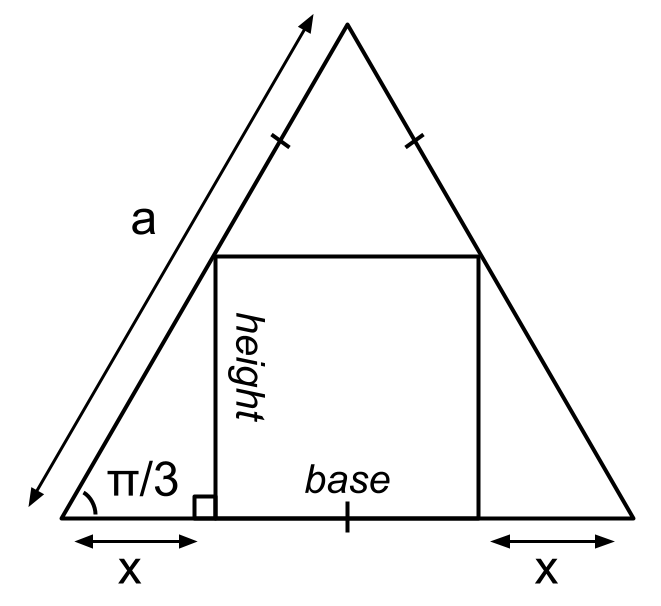
\includegraphics[scale = 0.32]{Q24 Diagram.png}
\end{center}

Now if we form an equation that represents the area of the rectangle 
before taking the derivative of this equation, we can find a global 
maximum. Let x be the distance between the leftmost corner of the diagram and the 
leftmost side of the rectangle. Since the triangle is equilateral, 
on the rightmost side there is another x. If we take the total base 
of the triangle, a, and subtract 2x out, we get the base of the rectangle.

$$base = a - 2x \text{\space \space \textbf{(1)}}$$

For the height of the rectangle, first consider the 30-60-90 triangle 
where the 60 degrees is labeled in the diagram. Since we know the angle 
and the base of the triangle is x, we can use tan(x) to find the height.

\addtolength{\jot}{-0.6em}
\begin{align*}
    tan(\theta) &= \dfrac{opp}{adj} \\
    tan \left( \dfrac{\pi}{3} \right) &= \dfrac{height}{x} && \theta = \dfrac{\pi}{3}, adj = x, opp=height \\
    x \times tan \left( \dfrac{\pi}{3} \right) &= height && \text{multiply x on both sides} \\
    \sqrt3 x&= height && \textbf{(2)} \text{\space \space By special triangle, } tan \left( \dfrac{\pi}{3} \right) = \sqrt3 \\
\end{align*}

\newpage

Now that we know the base and height of the rectangle, we can calculate 
create an equation to express the area before finding the derivative and 
the global maximum. Let A be area.

\addtolength{\jot}{-0.6em}
\begin{align*}
    A &= base \times height && \text{Area of a rectangle}\\
    A &= (a - 2x)(\sqrt3x) && \textbf{(3)} \text{\space \space Sub (1) and (2) in as base and height} \\
    A &= \sqrt3ax-2\sqrt3x^2 && \text{Expand} \\
    A' &=  \sqrt3a-4\sqrt3x && \textbf{(4)} \text{\space \space Use Power Rule, get derivative} \\
    0 &=  \sqrt3a-4\sqrt3x && \text{Solve for A' = 0 for critical points}\\
    4\sqrt3x &=  \sqrt3a && \text{Add } 4\sqrt3x \text{ to both sides} \\
    4x &=  a && \text{Divide } \sqrt3 \text{ from both sides} \\
    x &= \dfrac{a}{4} && \text{Divide } 4 \text{ from both sides} \\  
\end{align*}

Now that we have a critial number, we need to test to see 
if it the value really is the absolute maximum. Apply product rule 
to (4) again to get the second derivative for a second derivative test.

\addtolength{\jot}{-0.6em}
\begin{align*}
    A' &=  \sqrt3a-4\sqrt3x && \textbf{(4)} \\
    A'' &=  -4\sqrt3 && \text{Apply product rule}\\
\end{align*}

The second derivative is always negative. This means at x = a/4, 
according to the second derivative test, the point will be the 
relative maximum. Also thinking logically for a moment, the area 
equation is a negative quadtratic meaning the vertex (which we 
found) will be the highest point.

\vspace{0.5cm}
\textbf{Solution continues on next page}

\newpage

\vspace{0.5cm}
Now we know that the maximum area is achieved at x = a/4. Now we 
can plug this back into the area equation to get the maximum area. Use (3).

\addtolength{\jot}{0.5em}
\begin{align*}
    A &= (a - 2x)(\sqrt3x) && \textbf{(3)} \\
    A &= \left(a - 2\times\dfrac{a}{4}\right)\left(\sqrt3\times\dfrac{a}{4}\right) && x=\dfrac{a}{4} \\
    A &= \left(a - \dfrac{a}{2}\right)\left(\dfrac{\sqrt3a}{4}\right) && \text{Simplify} \\
    A &= \left(\dfrac{2a}{2} - \dfrac{a}{2}\right)\left(\dfrac{\sqrt3a}{4}\right) && \text{get Same Denominator} \\
    A &= \left(\dfrac{a}{2}\right)\left(\dfrac{\sqrt3a}{4}\right) && \text{Simplify} \\
    A &= \dfrac{\sqrt3a^2}{8} \\
\end{align*}

$$\boxed{\therefore \text{\space the maximum area is } \dfrac{\sqrt3a^2}{8} }$$

\newpage

\end{enumerate}
\end{document} 
